\chapter{Tvorba aplikace}
\label{4-tvorba-aplikace}

\section{Vytvoření základní aplikace}

Aplikace, která byla vytvořena v projektu FGIS nebyla vytvořena
správně, a obsahovala zbytečně složitý, a chybný kód. Začalo se tedy
od začátku. Nejprve byla vytvořen projekt příkazem \emph{django-admin
  startproject mysite}. V projektu následně byla vytvořena aplikace
pomocí \emph{python manage.py startapp}. Aplikace byla v
\emph{settings.py} přidána do \textbf{INSTALLED\_APPS}. Dále se
nastavilo připojení k databázi. V \emph{settings.py} se tedy v
\textbf{DATABASES} se změnil engine na MySQL, protože Django v základu
používá SQLite. Změnilo se ještě NAME, USER, PASSWORD, HOST A PORT,
protože databáze byla provozována na školním serveru
geo102.fsv.cvut.cz. Po připojení se musel vygenerovat model databáze,
příkazem inspectdb, viz. Instalace a inicializace projektu. Dále byla
provedena migrace, aby se v databázi vytvořily Django
tabulky. Posledním krokem bylo vytvoření superuživatele, který se bude
moci přihlásit do naší i administrátorské aplikace. To bylo
realizováno příkazem \emph{python manage.py createsuperuser}.

Na stránce GitLab byl vytvořen nový repozitář, do kterého se celý
projekt přesunul a nadále v něm byl průběžně zálohován. Dále se tam
vytvářely tzv. \emph{issues}, kde se plánovaly nadcházející úkoly při
tvorbě aplikace.

\section{Tvorba aplikace v uživatelském prostředí}

Prvním větším úkolem bylo vytvořit aplikace, která bude zobrazovat
data, a po přihlášení je bude moci uživatel také přidávat, mazat a
editovat. Nejprve se tady do adresáře aplikace přidala soubor urls.py,
který se následně připojil do projektového adresáře urls.py. Tento
způsob je výhodný při použití více aplikace, kdy si každá aplikace
uchovává své url adresy a projekt je tak přehlednější. Pokračovalo se
vytvořením pohledů založených na třídách, které se v Pythonu používají
pro nahrazení pohledů jako funkcí. Použity jsou základní pohledy jako
ListView pro zobrazení obsahu tabulky nebo CreateView pro uložení dat
do databáze. V aplikaci v soubory \emph{views.py} jsou tedy vytvořeny
třídy pohledů pro každou url adresu. Definice těchto tříd vypadá
následovně \emph{class “název třídy“(Listview):} dále se u třídy
definuje model, který se má zobrazit a template\_name neboli název
šablony, která se použije při zobrazení.

\begin{figure}[H] \centering
    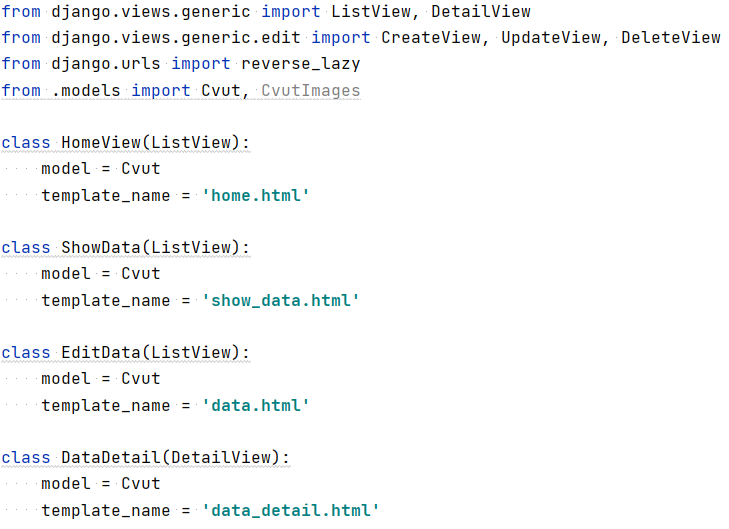
\includegraphics[width=350pt]{./pictures/6-nahled-views-aplikace.PNG}
    \caption[Náhled views.py a jeho tříd]{Náhled views.py a jeho tříd}
	\label{fig:Náhled views.py a jeho tříd}              
\end{figure}


V souboru \emph{urls.py} jsou propojeny url adresy, pohledy a html
šablony, na které se odkazují. Do urls.py musí být zároveň importovány
všechny použité pohledy. Dále se provede import \emph{path}. Poté se
sestaví \emph{urlpatterns}, což je seznam, který obsahuje jednotlivé
adresy. Ty jsou v něm uvedeny ve funkci path, která má dva povinné
argumenty, route a view a dva nepovinné, name a kwargs. Route uvádí
adresu, pod jakou se bude stránka načítat a view odkazuje na
importovaný pohled. Zde byla použita funkce \emph{as\_view()}, která
se používá, pokud je pohled typu třída. Jméno je uvedeno jako název
html šablony.

\begin{figure}[H] \centering
    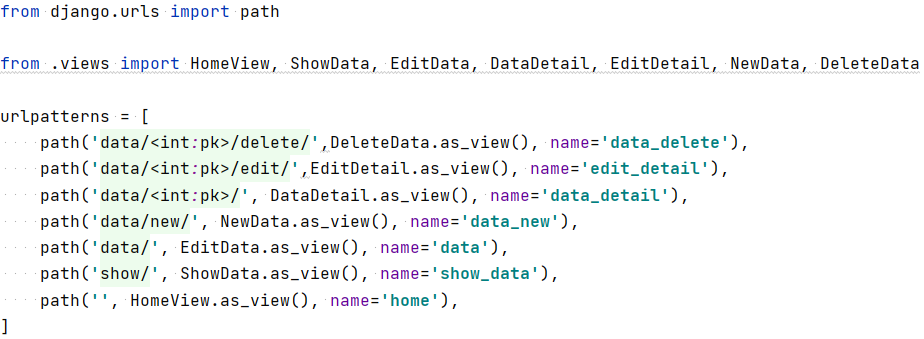
\includegraphics[width=450pt]{./pictures/7-urls-aplikace.PNG}
    \caption[Náhled urls.py v adresáři aplikaci]{Náhled urls.py v adresáři aplikaci}
	\label{fig:Náhled urls.py v adresáři aplikaci}              
\end{figure}

Pro vytvoření html šablon se vytvořila složka \emph{templates}, kde
jsou uloženy jednotlivé html soubory. Tato složka se v settings.py
nastaví jako výchozí pro jejich zobrazení. Poté se už mohou vytvářet
jednotlivé šablony. Šablony jsou vždy vytvořeny s podmínkou \emph{if
  user.is\_authenticated}, tedy pokud je uživatel přihlášen, zobrazí
se mu na stránce možnosti data editovat, vytvářet a mazat. S tímto je
spojena ještě další změna v \emph{settings.py}, kde je přidáno
\textbf{LOGIN\_REDIRECT\_URL = 'home'} a \textbf{LOGOUT\_REDIRECT\_URL
  = 'home'} které uživatele po přihlášení a odhlášení přesměruje na
domovskou stránku. Ve složce \emph{templates} je ještě složka
\emph{registration}, kde je umístěn \emph{login.html}. Html soubory
zobrazují data v základní formě tabulek a nejsou graficky upravována
pomocí css.

\begin{figure}[H] \centering
    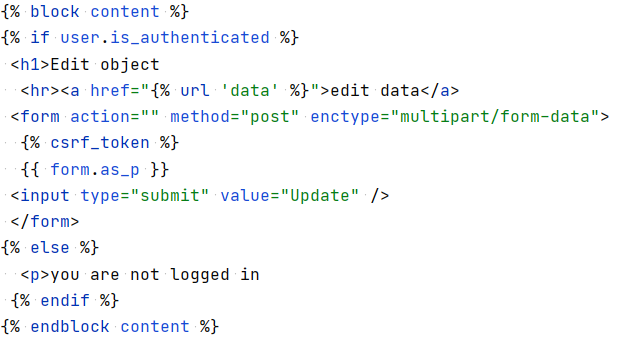
\includegraphics[width=350pt]{./pictures/8-edit-detail-html.PNG}
    \caption[Náhled html souboru edit detail]{Náhled html souboru edit detail}
	\label{fig:Náhled html souboru edit detail}
\end{figure}


\newpage

\section{Přidání obrázků}

Dalším úkolem bylo vyřešit přidávání obrázků k jednotlivým
záznamům. Obrázky by se neměly ukládat do databáze, ale do adresáře v
aplikaci. Databáze poté bude obsahovat cestu k těmto souborům. K tomu
byla vytvořena nová tabulka, který byla přes cizí klíč spojena s
tabulkou se záznamy. Tabulka byla vytvořena v modelu, a poté pomocí
migrací byl přenesena do databáze. Obsahuje tedy pole ID, což je
primární klíč tabulky, Post, který je cizím klíčem k tabulce Cvut a
sloupec Image, do kterého se zaznamenává cesta k danému souboru.

\begin{figure}[H] \centering
    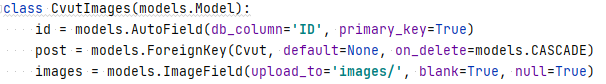
\includegraphics[width=430pt]{./pictures/9-db-cvutimages.PNG}
    \caption[Náhled tabulky CvutImages pro ukládání obrázků]{Náhled tabulky CvutImages pro ukládání obrázk}
	\label{fig:Náhled tabulky CvutImages pro ukládání obrázk}              
\end{figure}

V nastavení se dále určí rootovský adresář pro nahrávané soubory
\textbf{MEDIA\_ROOT = os.path.join(BASE\_DIR, 'media')} a
\textbf{MEDIA\_URL = '/media/'}.  A v poslední řadě se musí nastavit v
projektovém urls.py media soubory, které django samo neumí
zobrazovat. Zde se provede import settings a static a k urlpatterns se
připojí funkce static.

\begin{figure}[H] \centering
    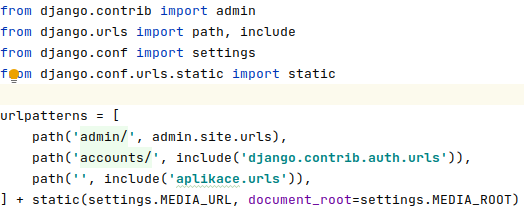
\includegraphics[width=350pt]{./pictures/10-media-urlspy.PNG}
    \caption[Náhled projektového urls.py]{Náhled projektového urls.py}
	\label{fig:Náhled projektového urls.py}              
\end{figure}

\newpage

\section{Statické soubory}

Pro řešení vizuální stránky webu jsou používány css soubory. Ve složce
aplikace se tedy vytvoří adresář static a tomu v \emph{settings} se
určí jeho nastavení pro statické soubory příkazy \textbf{STATIC\_URL =
  '/static/'} a \textbf{STATICFILES\_DIRS = [os.path.join(BASE\_DIR,
  'static')]}. Ve složce static je vytvořen adresář css, kde se
nachází základní css soubor base.css. Ten je ovšem prázdný a není
připojen k žádnému html souboru.

\section{Nastavení jazyka a času}

Dalším nastavením bylo použití našeho středoevropského času a českého
jazyka. Velice jednoduché nastavení, kdy v \emph{settings} je po
vytvoření aplikace nastaven jazyk na angličtinu a čas na UTC. Pro
změnu se tedy přepíše \textbf{LANGUAGE\_CODE = 'en-us'} na
\textbf{LANGUAGE\_CODE = 'cs'} a \textbf{TIME\_ZONE = 'UTC'} na
\textbf{TIME\_ZONE = 'CET'}.


\textcolor{red}{zadokrování aplikace} 

\section{Administrátorské prostředí}



















